\documentclass[11pt]{article}
\usepackage[margin=1in]{geometry}
\usepackage{booktabs}
\usepackage{graphicx}
\usepackage{amsmath}
\usepackage{amssymb}
\usepackage{microtype}

\title{Fine-tuning AlphaGenome on single-cell pseudobulk multiome data}
\author{}
\date{}

\begin{document}
\maketitle

\section{Summary}
One AlphaGenome model was fine-tuned jointly on five single-cell multiome
studies (ten species-specific sources, 20 output heads). The most effective
changes were to the training targets: RNA rebuilt as gene-level pseudobulk
counts per million (CPM) from raw counts, ATAC rebuilt from raw fragments where
released tracks were unsuitable, and removal of near-empty or unsupported cell
groups. A correlation term in the loss, staged head training, and low-rank
adapters gave smaller gains. The selected model reaches mean held-out
chromosome correlation $R=0.684$ for ATAC and $0.570$ for RNA. On fine-mapped
brain eQTLs, gene-span variant effects give AUROC $0.55$ (SingleBrain) and
$0.64$ (XQTL), with discrimination concentrated near the TSS and only small
gains from matching the eQTL cell type to its model track.

\section{Data}
Each study provides pseudobulk ATAC and RNA profiles for annotated cell groups
(Table~\ref{tab:data}). Each source keeps its own genome assembly, and
chromosomes 8 and 9 of each assembly are held out for validation and test.
Macaque and marmoset sequences use AlphaGenome's human organism embedding.

\begin{table}[ht]
\centering
\small
\caption{Training data. Group counts are ATAC/RNA cell groups; Liu and
Johansen RNA heads have one channel per strand. ATAC source is the released
track or a reconstruction from raw fragments.}
\label{tab:data}
\begin{tabular}{@{}lllll@{}}
\toprule
Study & Tissue & Species & Groups & ATAC source \\
\midrule
Mannens (HDA) & first-trimester brain & human & 134/134 & released \\
Liu (HDMA) & fetal, 12 organs & human & 186/186 & fragments \\
Johansen 2025 & basal ganglia & human, macaque, marmoset & 47/47 & fragments \\
Zemke 2023 & motor cortex & human, macaque, marmoset, mouse & 20/19 & released \\
Zemke 2024 & hippocampus (aging) & human & 18/18 & fragments \\
\bottomrule
\end{tabular}
\end{table}

\section{Training strategies}
Performance is measured by signed double-centered Pearson correlation $R$. For
target and prediction matrices $Y,\hat{Y}\in\mathbb{R}^{N\times C}$, with $N$
genomic elements (genes for RNA, 128 bp bins for ATAC) and $C$ cell groups, row
and column means are removed before computing the correlation, so $R$ measures
relative structure across elements and cell groups rather than assay scale.

\paragraph{RNA targets and loss.} Released coordinate RNA tracks were replaced
with gene-level targets. Raw counts are summed over the cells of each group
before CPM normalization; summing per-cell normalized expression instead gives
targets whose double-centered agreement with the correct ones is only
$0.46$--$0.54$ (Johansen). The model's RNA output $\hat{x}\in\mathbb{R}^{B\times
C}$ over $B$ 128 bp bins is read out per gene $g$ as \begin{equation}
\hat{y}_{g,c}=\sum_{b} w_{g,b}\,\hat{x}_{b,c},
\end{equation}
where $w_{g,b}\in[0,1]$ is the fraction of bin $b$ covered by exons of $g$,
and the loss is the squared error between $\log(1+\hat{y}_{g,c})$ and
$\log(1+y_{g,c})$. In a matched frozen-backbone comparison on Zemke 2023 that
changed only this target, test RNA $R$ rose from $0.152$ to $0.421$ (validation
$0.250$ to $0.360$) with ATAC unchanged. The gene-level target also avoids a
ribosomal-repeat artifact in the released marmoset tracks, where one 341 bp
window carried 71\% of the chromosome-9 RNA variance. Adding a per-bin
coverage loss did not help (HDA, mean validation $R$ $0.604$ with versus
$0.598$ without), so it was dropped.

\paragraph{ATAC targets.} Where released tracks were significance scores or
poorly matched coverage, ATAC was rebuilt from raw fragments as full-depth
fragment coverage per million fragments, without downsampling. For Johansen
human, test $R$ was $0.210$ with released tracks and $0.458$ with the rebuilt
target under the same training setup.

\paragraph{Cell-group quality control.} One Johansen group with 33,424
fragments (median $1.1\times 10^8$) contributed 48\% of all squared ATAC signal
and was removed. Groups without supporting cell assignments are masked rather
than given zero targets: four Zemke 2024 subtype channels and the Zemke 2023
L5 IT RNA group.

\paragraph{Loss.} A double-centered correlation term, $1-R$ computed within
each batch, was added to the loss of every RNA head (weight $1$, HDA $0.1$) and
of the Zemke 2023 ATAC heads (weight $3$). In a matched continuation of the
joint model it raised validation $R$ from $0.568$ to $0.583$, mainly through
RNA ($0.461$ to $0.491$). The effect varies by study; one weighting reduced
Liu RNA, which the final weights recover.

\paragraph{Model and optimization.} The pretrained backbone is shared by all
heads. Each source has its own ATAC and RNA heads, because target
distributions differ between species of the same study; with equal sampling
of sources this raised LoRA test $R$ from $0.584$ to $0.605$ relative to one
pooled head per study and modality, a comparison that changes both factors
together. Heads were first trained for 12 epochs on a frozen backbone,
initialized from the pretrained neural accessibility tracks of matching cell
types; at epoch 4 this initialization gave validation $R$ $0.507$ against
$0.488$ for random initialization. Adapters were then trained from these heads:
LoRA (rank 16) on attention and pair projections, plus LoCon (rank 4) on
downsampling blocks 2--5, at learning rate $3\times10^{-4}$. Broad LoCon
improved test $R$ by $0.008$ and $0.005$ in two of three matched comparisons
and was neutral in the third. Learning rate $10^{-3}$ was unstable for LoCon.

\paragraph{Not helpful.} Higher adapter rank (LoRA 32, LoCon 8), uniform RNA
loss upweighting, target value transforms, refitting heads after adapter
training, and gene-balanced batch ordering did not improve held-out $R$.

\section{Held-out chromosome results}
The selected checkpoint (LoRA+LoCon, epoch 21) uses the targets above with
Zemke 2024 ATAC rebuilt from fragments. Table~\ref{tab:heldout} lists test
$R$ per source. Mean validation and test $R$ are $0.585$ and $0.627$ (ATAC
$0.665$/$0.684$, RNA $0.504$/$0.570$). Split-half reliability gives correlation
ceilings of $0.82$--$0.93$ for Johansen ATAC and $0.90$ for Zemke 2024 ATAC,
so those ATAC results are near the noise limit, whereas RNA targets have
ceilings of $0.93$ or higher where measured and remain well below them.

A matched run with released Zemke 2024 ATAC tracks reached test $R$ $0.603$.
The two runs differ only in that one head, but most of the difference comes
from other heads (for example Zemke 2023 mouse RNA, $0.311$ against $0.603$),
so differences of a few hundredths in mean $R$ between single runs should not
be over-interpreted.

\begin{table}[ht]
\centering
\small
\caption{Test-chromosome $R$ of the selected model.}
\label{tab:heldout}
\begin{tabular}{@{}llrr@{}}
\toprule
Study & Species & ATAC & RNA \\
\midrule
HDA & human & 0.817 & 0.660 \\
Liu & human & 0.784 & 0.485 \\
Johansen 2025 & human & 0.644 & 0.584 \\
 & macaque & 0.463 & 0.524 \\
 & marmoset & 0.600 & 0.453 \\
Zemke 2023 & human & 0.743 & 0.572 \\
 & macaque & 0.663 & 0.679 \\
 & marmoset & 0.615 & 0.649 \\
 & mouse & 0.739 & 0.610 \\
Zemke 2024 & human & 0.769 & 0.484 \\
\midrule
Mean & & 0.684 & 0.570 \\
\bottomrule
\end{tabular}
\end{table}

\section{Fine-mapped eQTL benchmark}
Positives are variants with posterior inclusion probability (PIP) above
$0.75$ and negatives have PIP below $0.01$, within 512 kb of the gene's TSS.
SingleBrain has 35 fine-mapping panels in seven brain cell classes (54,193
variants); XQTL has six cell-type panels (10,452 variants). Each variant is
scored with the human Zemke 2023 RNA head on a 1 Mb window centered at the
TSS. The gene-span effect is the absolute alternate-minus-reference
difference in mean prediction over the gene's bins, averaged over the tracks
matched to the panel's cell type. The TSS-bin summary performs worse and is
not shown.

Table~\ref{tab:eqtl} compares the selected model with the head-only model and
two adapter models that use the released Zemke 2024 ATAC tracks, and with one
selected pretrained AlphaGenome track per cell type. Trained models differ by
at most $0.015$ in pooled AUROC, close to the variation of about $0.005$
between repeated runs. The native tracks were selected on the same variants,
so their values are optimistic. Discrimination is concentrated near the TSS:
gene-span AUROC is $0.64$--$0.70$ (SingleBrain) and $0.81$--$0.87$ (XQTL)
within 1 kb, and falls below $0.5$ for all models beyond about 50 kb
(SingleBrain) and 100 kb (XQTL) (Figure~\ref{fig:distance}).

\begin{table}[ht]
\centering
\small
\caption{Gene-span eQTL discrimination. AUROC and AP are pooled over panels;
``within'' is the mean of per-cell-class AUROC.}
\label{tab:eqtl}
\begin{tabular}{@{}lrrrrrr@{}}
\toprule
 & \multicolumn{3}{c}{SingleBrain} & \multicolumn{3}{c}{XQTL} \\
\cmidrule(lr){2-4}\cmidrule(lr){5-7}
Model & AUROC & AP & Within & AUROC & AP & Within \\
\midrule
Head-only & 0.547 & 0.444 & 0.550 & 0.635 & 0.608 & 0.644 \\
LoRA & 0.540 & 0.432 & 0.539 & 0.628 & 0.600 & 0.642 \\
LoRA+LoCon & 0.540 & 0.434 & 0.542 & 0.637 & 0.615 & 0.643 \\
Selected (LoRA+LoCon, raw Zemke 2024 ATAC) & 0.547 & 0.445 & 0.545 & 0.643 & 0.623 & 0.646 \\
Native matched tracks & 0.524 & 0.439 & 0.535 & 0.627 & 0.626 & 0.650 \\
\bottomrule
\end{tabular}
\end{table}

\begin{figure}[ht]
\centering
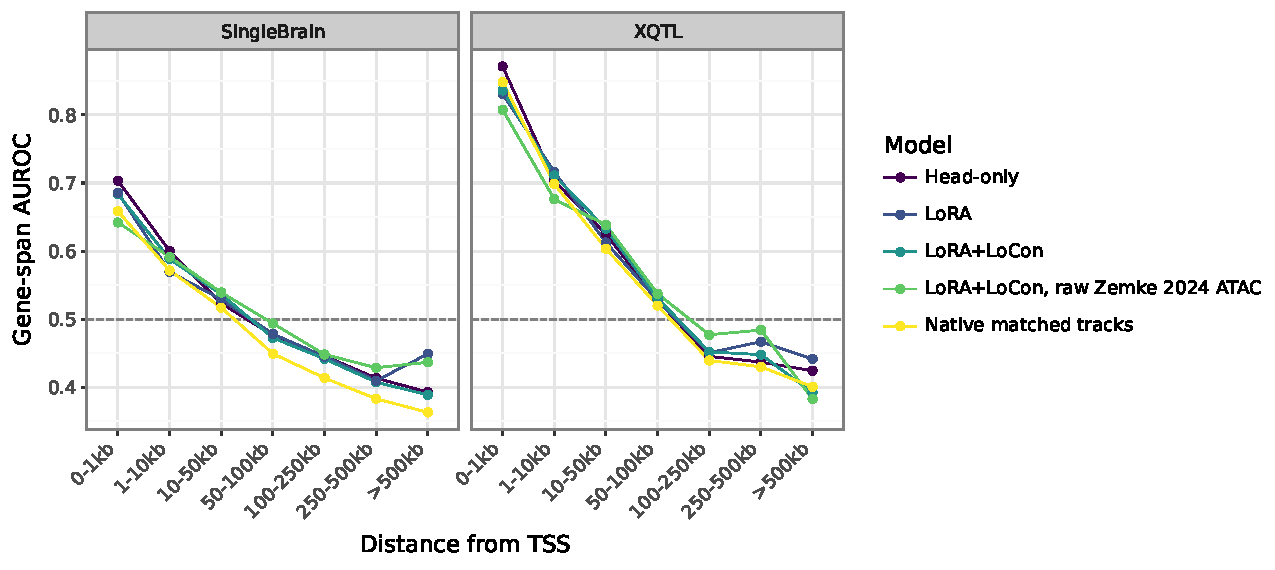
\includegraphics[width=\linewidth]{figures/v0data_gene_span_auroc_by_distance.pdf}
\caption{Gene-span AUROC by distance between variant and TSS. The dashed line
is chance.}
\label{fig:distance}
\end{figure}

The trained tracks carry a small amount of cell-type-specific signal. Scoring
each panel with every cell class's tracks, the matched class exceeds the
unmatched ones by $0.024$--$0.032$ AUROC on SingleBrain and $0.033$--$0.057$ on
XQTL, which is significant under permutation of the class assignment for
every model. The effect is driven by microglia (XQTL AUROC $0.69$--$0.73$ with
microglia tracks against at most $0.63$ with other tracks), astrocytes, and
oligodendrocytes; excitatory and inhibitory neuron panels show little
specificity. Predicted effects are largely shared across cell types, with
median Spearman correlation $0.63$--$0.69$ between tracks.

\end{document}
